\documentclass[draft]{beamer}
\usetheme{Warsaw}
\usepackage{ifdraft}
\usepackage{standalone}
\usepackage{lmodern} % Allows arbitrary font sizes to prevent warnings.
\usepackage{tikz}
\usetikzlibrary{patterns}
\usetikzlibrary{calc}
\definecolor{printred}{RGB}{215,25,28}
\definecolor{printorange}{RGB}{253,174,97}
\definecolor{printyellow}{RGB}{255,255,191}
\definecolor{printgreen}{RGB}{171,221,164}
\definecolor{printblue}{RGB}{43,131,186}
\title{CASCADE}
\subtitle{FPGA Stencil Code Implementation Pattern}
\author{Stephen~Roberts}
\institute{The University Of Warwick}

\begin{document}
  \frame{\titlepage}
  \begin{frame}
    \frametitle{Stencil Codes}
    \begin{figure}
      \centering
      % https://www.sharelatex.com/blog/2013/08/27/tikz-series-pt1.html

\documentclass[tikz]{standalone}
\begin{document}
\newcommand{\drawstencil}[2]{%
  \fill[red!30!white] (#1-1,#2) rectangle (#1+2,#2+1);
  \fill[red!30!white] (#1,#2-1) rectangle (#1+1,#2+2);
}
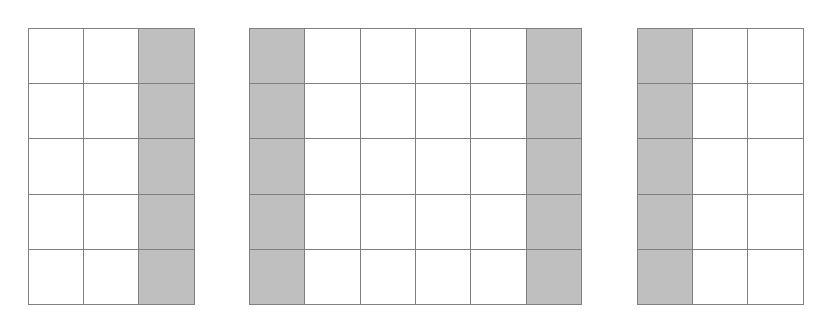
\begin{tikzpicture}[x=2em,y=2em]

  \fill[lightgray](-2,0) rectangle (-1, 5);
  \fill[lightgray] (0,0) rectangle (1,5);
  \fill[lightgray] (5,0) rectangle (6,5);
  \fill[lightgray](7,0) rectangle (8, 5);

  \drawstencil{2}{2}

  \draw[step=1, gray, very thin] (-4,0) grid (-1, 5);
  \draw[step=1, gray, very thin] (0,0) grid (6, 5);
  \draw[step=1, gray, very thin] (7,0) grid (10, 5);

\end{tikzpicture}
\end{document}

    \end{figure}
  \end{frame}

  \begin{frame}
    \frametitle{Stencil Codes - Decomposition}
    \begin{figure}
      \centering
      % https://www.sharelatex.com/blog/2013/08/27/tikz-series-pt1.html

\documentclass[tikz]{standalone}
\usetikzlibrary{patterns}
\begin{document}
\newcommand{\drawstencil}[2]{%
  \draw[darkgray, thick, pattern=north west lines, pattern color=gray] (#1-1, #2) rectangle (#1+2, #2+1);
  \draw[darkgray, thick, pattern=north west lines, pattern color=gray] (#1, #2-1) rectangle (#1+1, #2+2);
  \draw[darkgray, thick, pattern=north east lines, pattern color=gray](#1, #2) rectangle (#1+1, #2+1);
}
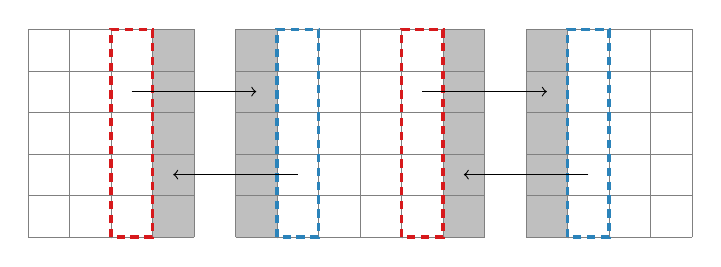
\begin{tikzpicture}[x=1.5em,y=1.5em]

  \fill[lightgray](-2,0) rectangle (-1, 5);
  \fill[lightgray] (0,0) rectangle (1,5);
  \fill[lightgray] (5,0) rectangle (6,5);
  \fill[lightgray](7,0) rectangle (8, 5);

  % Grids
  \draw[step=1, gray, very thin] (-5,0) grid (-1, 5);
  \draw[step=1, gray, very thin] (0,0) grid (6, 5);
  \draw[step=1, gray, very thin] (7,0) grid (11, 5);

  \onslide<1> {
    \drawstencil{1}{2} 
  }
  \onslide<2> {
    % Left-To-Right transmission (->)
    \draw[printred, densely dashed, very thick](-3,0) rectangle (-2, 5);
    \draw[->] (-2.5,3.5) -- (0.5,3.5);
    \draw[printred, densely dashed, very thick](4,0) rectangle (5, 5);
    \draw[->] (4.5,3.5) -- (7.5,3.5);

    % Right-To-Left transmission (<-)
    \draw[printblue, densely dashed, very thick] (1,0) rectangle (2,5);
    \draw[->] (1.5, 1.5) -- (-1.5, 1.5);
    \draw[printblue, densely dashed, very thick] (8,0) rectangle (9,5);
    \draw[->] (8.5, 1.5) -- (5.5, 1.5);
  }

\end{tikzpicture}
\end{document}

    \end{figure}
  \end{frame}

  \begin{frame}
    \frametitle{Stencil Codes - Boundary Exchanges}
    \begin{figure}
      \centering
      % https://www.sharelatex.com/blog/2013/08/27/tikz-series-pt1.html

\documentclass[tikz]{standalone}

\definecolor{printred}{RGB}{215,25,28}
\definecolor{printorange}{RGB}{253,174,97}
\definecolor{printyellow}{RGB}{255,255,191}
\definecolor{printgreen}{RGB}{171,221,164}
\definecolor{printblue}{RGB}{43,131,186}
\begin{document}
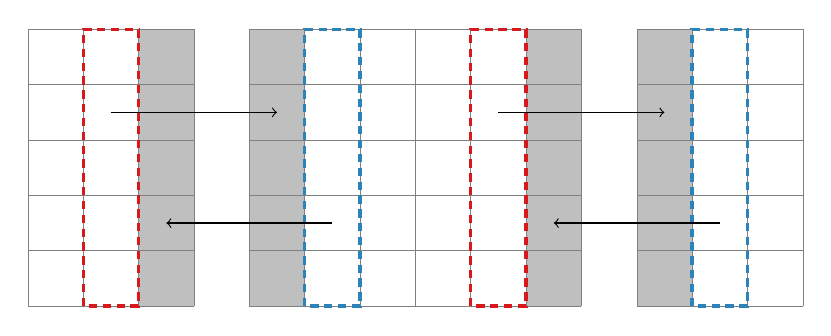
\begin{tikzpicture}[x=2em,y=2em]

  % Ghost Cells
  \fill[lightgray](-2,0) rectangle (-1, 5);
  \fill[lightgray] (0,0) rectangle (1,5);
  \fill[lightgray] (5,0) rectangle (6,5);
  \fill[lightgray](7,0) rectangle (8, 5);

  % Grids
  \draw[step=1, gray, very thin] (-4,0) grid (-1, 5);
  \draw[step=1, gray, very thin] (0,0) grid (6, 5);
  \draw[step=1, gray, very thin] (7,0) grid (10, 5);

  % Left-To-Right transmission (->)
  \draw[printred, densely dashed, very thick](-3,0) rectangle (-2, 5);
  \draw[->] (-2.5,3.5) -- (0.5,3.5);
  \draw[printred, densely dashed, very thick](4,0) rectangle (5, 5);
  \draw[->] (4.5,3.5) -- (7.5,3.5);

  % Right-To-Left transmission (<-)
  \draw[printblue, densely dashed, very thick] (1,0) rectangle (2,5);
  \draw[->] (1.5, 1.5) -- (-1.5, 1.5);
  \draw[printblue, densely dashed, very thick] (8,0) rectangle (9,5);
  \draw[->] (8.5, 1.5) -- (5.5, 1.5);

\end{tikzpicture}
\end{document}

    \end{figure}
  \end{frame}
  \ifdraft{\def \stencilradius{1}}{\def \stencilradius{6}}
  % https://www.sharelatex.com/blog/2013/08/27/tikz-series-pt1.html

\documentclass[beamer]{standalone}
\usepackage{lmodern}
\usepackage{tikz}
\usetikzlibrary{calc}
\def \stencilradius{6}
\begin{document}
\begin{frame}
  \frametitle{Stencil Codes - Dependency Propagation}
  \begin{figure}
    \centering
    \begin{tikzpicture}[x=1em,y=1em]
      \def \maxrow {16}
      \def \maxcol {16}
      \def \originx{8}
      \def \originy{8}
      
      \foreach \sr in {1,...,\stencilradius}
      {
        \foreach \layer in {\sr,...,1}
        {
          \foreach \r in {0,...,\maxrow}
          {
            \foreach \c in {0,...,\maxcol}
            {
              \pgfmathparse{int(abs(\r - \originx) + abs(\c - \originy))}
              \ifnum \pgfmathresult < \layer
              \pgfmathparse{(\sr - \layer) * 15}
                \fill<\sr>[black!\pgfmathresult!lightgray] (\r,\c) rectangle (\r+1,\c+1);
              \fi
            }
          }
        }
      }
      \draw[step=1, gray, very thin] (0,0) grid (\maxrow+1, \maxcol+1);
    \end{tikzpicture}
  \end{figure}
\end{frame}
\end{document}

 
\end{document}
